\subsection{Task2 New Gripper Design}
The last gripper in task 2 our humanoid robot have to fit the wrench into the shaft and rotate $360$ degrees by move the arm and solve the inverse kinematics. However, sometimes(usually) the inverse kinematics can not be solved due to the limitation of the arm. In the first report we attempt to rotate the wrench $4$ times with $90$ degrees each time. This is very time consuming and now we designed a new gripper that use the servo motor attached to the gripper which can directly robot $360$ degrees and capable of the torque $5Nm$. 

As Fig. \ref{gripper} shows, the gripper consists of a servo motor and a attachment with magnets. We choose Dynamixel MX-106 servo motor which has a high stall torque of $8.4 Nm$. Under the situation of $5 Nm$ torque load, it can rotate at a speed of more than $10 rpm$, which saves a lot of time to rotate the shaft. To pick and align the wrench into the shaft, we equipped a spring to the gripper attachment. The spring pushes the central stick so that when we pick the wrench, the wrench's one size will fit into the stick. To align the wrench to the shaft, we only need to align the central stick to the shaft and push the gripper toward to the panel, the spring attached to the gripper will be compressed which will result in the wrench being pushed into the shaft. Then directly control the Dynamixel motor will rotate the shaft easily. We need more experiments to validate the feasibility of this gripper and then we can decide whether to equip this kind of gripper in the final or not.

 \begin{figure}%[hb]
    \begin{center}
    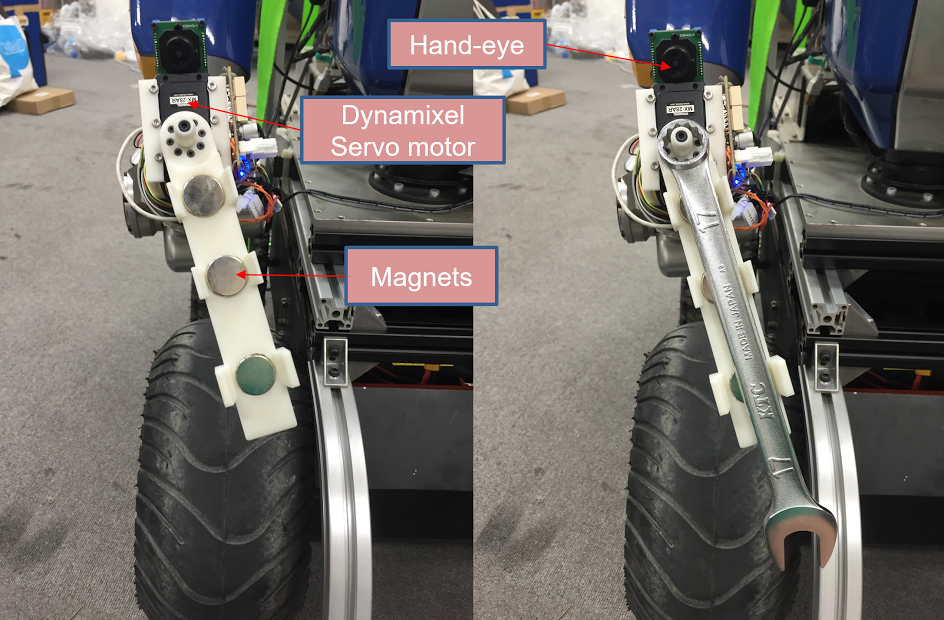
\includegraphics[keepaspectratio=true, width=1\linewidth, height=0.3\textheight]{sections//task2//images//gripper.png}
      \end{center}
    \caption{New Gripper Design}
    \label{gripper}
 \end{figure}

